\lecture{11}{29. September 2025}{Internal Flows: Flows in Pipes and Ducts}

\subsection{Shear Stress Distribution in Fully Developed Pipe Flow}
We, once again, consider fully developed flow in a horizontal circular pipe, except this time the flow is not restricted to being laminar. Above it was shown that a force balance between friction and pressure forces leads to
\[ 
\tau_{rx} = \frac{r}{2} \left( \frac{\mathrm{d}p}{\mathrm{d}x}  \right) + \frac{c_1}{r}
.\]
As we cannot have infinite stress at the centerline, $c_1$ must be zero, so
\[ 
\tau_{rx} = \frac{r}{2} \frac{\mathrm{d}p}{\mathrm{d}x} 
.\]
This indicates that for both laminar and turbulent fully developed flows the shear stress varies linearly across the pipe from zero at the centerline to a maximum at the pipe wall. 

Turbulent flow is represented at each point in time by a mean velocity $\overline{u}$ plus randomly fluctuating velocity components $u'$ and $v'$ in the $x$ and $y$ directions respectively. 
These components continuously transfer momentum between adjacent fluid layers, tending to reduce any velocity gradient present.
This results in an apparent stress termed the \textit{Reynolds stress} given by $- \rho \overline{u'v'}$.
In terms of distance from the wall, the total stress in turbulent flow can be written as
\begin{equation}\label{eq:totstreturb}
  \tau = \tau_{\mathrm{lam}} + \tau_{\mathrm{turb}} = \mu \frac{\mathrm{d}\overline{u}}{\mathrm{d}y} - \rho \overline{u'v'}
\end{equation}
In the above, the fluctuations $u'$ and $v'$ are negatively correlated, so that $\tau_{\mathrm{turb}}= - \rho \overline{u'v'}$ is positive. 
On \Cref{fig:f8_8} experimental measurements of the Reynolds stress for two fully developed turbulent pipe flows are plotted.

\begin{figure} [ht]
  \centering
  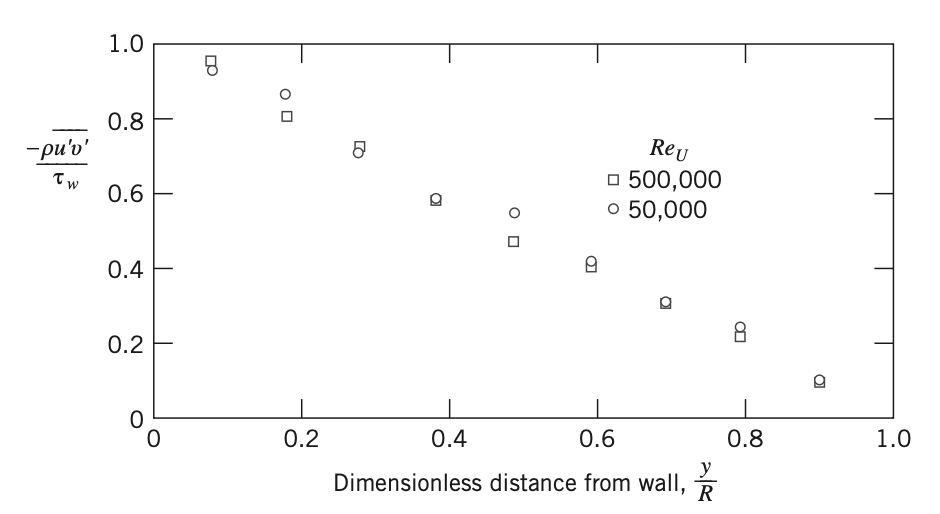
\includegraphics[width=0.5\linewidth]{./figures/f8_8.png}
  \caption{Turbulent shear stress (Reynold's stress) for fully developed turbulent flow in a pipe.}
  \label{fig:f8_8}
\end{figure}


\subsection{Turbulent Velocity Profiles in Fully Developed Pipe Flow}
We consider the relation for the total stress in turbulent flow from \Cref{eq:totstreturb} and divide by the density to get
\[ 
\frac{\tau}{\rho} = \nu \frac{\mathrm{d} \overline{u}}{\mathrm{d}y} - \overline{u'v'}
.\]
It is convenient to consider the turbulent fluctuations in the mean velocity as a result of a small element of fluid moving upward a small distance $\mathcal{l}$ into a region of higher velocity.
The fluctuating velocity $u'$ is then negative and given by
\[ 
u' = - \mathcal{l} \frac{\mathrm{d}\overline{u}}{\mathrm{d}y} 
\]
where $\mathcal{l}$ is the so-called mixing length. Similarly for the $v$ component of velocity
\[ 
v' = \mathcal{l} \frac{\mathrm{d}\overline{v}}{\mathrm{d}x} 
.\]
In homogeneous turbulence $u'$ and $v'$ are equal and therefore
\[ 
v' = u' = \mathcal{l} \frac{\mathrm{d}\overline{u}}{\mathrm{d}y} 
.\]

The turbulent shear stress is then approximated by
\[ 
\frac{\tau_{\mathrm{turb}}}{\rho} = \mathcal{l}^2 \left( \frac{\mathrm{d}\overline{u}}{\mathrm{d}y}  \right)^2
.\]

Furthermore, the mixing length approximately increases in proportion to the distance from the wall,
\[ 
\mathcal{l} = ky
.\]

In general, the velocity profile for turbulent flow through a smooth pipe may be approximated by the power-law equation
\[ 
\frac{\overline{u}}{U} = \left( \frac{y}{R} \right)^{\frac{1}{n}} = \left( 1 - \frac{r}{R} \right)^{\frac{1}{n}}
\]
where the exponent $n$ varied with the Reynold's number and is approximately
\[ 
n = \num{-1,7} +\num{1,8} \, \log \mathrm{Re}_U
\]
for $\mathrm{Re}_U > \num{2e4}$. 


\subsection{Energy Considerations in Pipe Flow}
In \Cref{sec:egl} the Energy Grade Line (EGL) was introduced,
\[ 
\mathrm{EGL} = \frac{p}{\rho g} + \frac{V^2}{2g} + z
.\]
This can be thought of as the total mechanical energi per unit mass in a flow.
This is constant for inviscid flow as there is no friction to dissipate the mechanical energy.
For viscous flow, however, friction will lead to a continuously decreasing EGL.

\begin{figure} [ht]
  \centering
  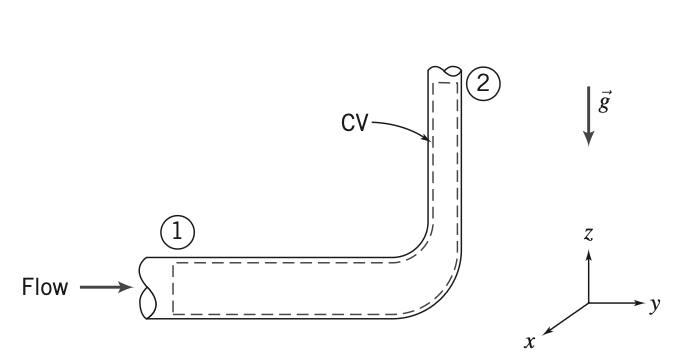
\includegraphics[width=0.5\linewidth]{./figures/f8_12.png}
  \caption{Control volume and coordinates for energy analysis through a \ang{90} reducing elbow.}
  \label{fig:f8_12}
\end{figure}

We consider the steady flow through the reducing elbow on \Cref{fig:f8_12}. 

The first law of thermodynamics is
\[ 
\dot{Q} - \dot{W}_s - \dot{W}_{\mathrm{shear}} -  \dot{W}_{\mathrm{other}} = \frac{\partial }{\partial t}  \int_{\mathrm{CV}} e \rho \, \mathrm{d}V + \int_{\mathrm{CS}} \left( e + p v \right)\rho \Vec{V} \cdot \mathrm{d}\Vec{A}
\]
where
\[ 
e = u + \frac{V^2}{2} + gz
.\]

For the elbow we assume that no shaft work and no other work is exerted, hence $\dot{W}_s = \dot{W}_{\mathrm{other}} = 0$.
Due to the no-slip condition the velocities at the walls will be zero so no shear work will be made even though shear forces are present at the walls.
Furthermore, we assume steady and incompressible flow and uniform internal energy and pressure at cross sections 1 and 2.

Under these assumptions the first law of thermodynamics for the system reduces to
\[ 
\dot{Q} = \dot{m} \left( u_2 - u_1 \right) + \dot{m} \left( \frac{p_2 - p_1}{\rho} \right) + \dot{m} g \left( z_2 - z_1 \right) + \int_{A_2} \frac{V_2^2}{2} \rho V_2 \, \mathrm{d}A_2 - \int_{A_1} \frac{V_1^2}{2}\rho V_1 \, \mathrm{d}A_1
.\]

\subsubsection{Kinetic Energy Coefficient}
We now define the \textit{kinetic energy coefficient}, $\alpha$, such that the product of this coefficient and the kinetic energy based on the average velocity equals the kinetic energy,
\[ 
\int_A \frac{V^2}{2} \rho V \, \mathrm{d}A = \alpha \int_A \frac{\overline{V}^2}{2} \rho V \, \mathrm{d}A = \alpha \dot{m} \frac{\overline{V}^2}{2}
\]
or
\[ 
\alpha = \frac{\int_A \rho V^3 \, \mathrm{d}A}{\dot{m} \overline{V}^2}
.\]
This can in many ways be thought of as a correction factor that allows us to use the average velocity $\overline{V}$ in the energy equation to compute the kinetic energy at a given cross section.

For laminar flow in a pipe, $\alpha = \num{2,0}$.

For turbulent pipe flow $\alpha$ can be determined as
\[ 
\alpha = \left( \frac{U}{\overline{V}} \right)^3 \frac{2n^2}{\left( 3+n \right)(3+2n)}
\]
where $n$ is the power law exponent.
For ``normal'' $n = 7$ power profiles $\alpha = \num{1,06}$.
Therefore $\alpha = 1$ is oftentimes a good approximation in pipe flow calculations.

\subsubsection{Head Loss}
Using the definition of $\alpha$ the first law of thermodynamics can be written
\[ 
\dot{Q} = \dot{m} \left( u_2 - u_1 \right) + \dot{m} \left( \frac{p_2 - p_1}{\rho} \right) + \dot{m} g \left( z_2 - z_1 \right) + \dot{m} \left( \frac{\alpha_2 \overline{V}_2^2}{2} - \frac{\alpha_1 \overline{V}_{1}^2}{2} \right)
.\]
Dividing by the mass flow rate gives
\[ 
\frac{\delta Q}{\mathrm{d}m} = u_2 - u_1 + \frac{p_2 - p_1}{\rho} + gz_2 - gz_1 + \frac{\alpha_2 \overline{V}_2^2}{2} - \frac{\alpha_1 \overline{V}_1^2}{2}
.\]
Rearranging this equation, we get
\begin{equation} \label{eq:828}
 \left( \frac{p_1}{\rho} + \alpha_1 \frac{\overline{V}_1^2}{2} + gz_1 \right) - \left( \frac{p_2}{\rho} + \alpha_2 \frac{V_2^2}{2} + gz_2 \right) = \left( u_2 - u_1 \right) - \frac{\delta Q}{\mathrm{d}m}
\end{equation}
In \Cref{eq:828} the term $\left( \frac{p}{\rho} + \alpha \frac{\overline{V}^2}{2} + gz \right)$ represents the mechanical energy per unit mass at a cross section.
The term $u_2 - u_1 - \frac{\delta Q}{\mathrm{d}m}$ is the difference in mechanical energy per unit mass between sections 1 and 2.
It represents the irreversible conversion of mechanical energy from section 1 to thermal energy at section 2.
We identify this group of terms as the total energy loss per unit mass and designate it by $h_{l_T}$.
Then,
\begin{equation}\label{eq:headloss}
  \left( \frac{p_1}{\rho} + \alpha_1 \frac{\overline{V}_1^2}{2} + gz_1 \right) - \left( \frac{p_2}{\rho} + \alpha_2 \frac{\overline{V}_2^2}{2} + gz_2 \right) = h_{l_T}
\end{equation}
\Cref{eq:headloss} allows us to compute the friction loss between two sections of pipe. 


\subsection{Calculation of Head Loss}
Total head loss, $h_{l_T}$, is the sum of major losses, $h_l$ due to frictional effects in the fully developed flow and minor losses $h_{l_m}$ resulting from entrances, fittings, and so on.

\subsubsection{Major Losses: Friction Factor}
We can use the energy balance in \Cref{eq:headloss} to evaluate the major head loss.
For fully developed flow through a constant area pipe, \Cref{eq:headloss} reduces to
\begin{equation}\label{eq:headlosssimple}
  \frac{p_1 - p_2}{\rho} = g \left( z_2 - z_1 \right) + h_l
\end{equation}
For a horizontal pipe, $z_2 = z_1$, and \Cref{eq:headlosssimple} reduces to
\begin{equation}\label{eq:headlossflat}
  \frac{p_1 - p_2}{\rho} = \frac{\Delta p}{\rho} = h_l
\end{equation}
Therefore, the major head loss can be expressed as the pressure loss for fully developed flow through a horizontal pipe of constant area.


\subsubsection{a. Laminar Flow}
In laminar flow, it has previously been shown that the pressure drop may be computed analytically for fully developed flow in a horizontal pipe, as
\[ 
\Delta p = 32 \frac{L}{D} \frac{\mu \overline{V}}{D}
.\]
Substituting in \Cref{eq:headlossflat} yields
\begin{equation}\label{eq:lamflowheadloss}
  h_l = 32 \frac{L}{D} \frac{\mu \overline{V}}{\rho D} = \frac{L}{D} \frac{\overline{V}^2}{2} \left( 64 \frac{\mu}{\rho \overline{V} D} \right) = \frac{64}{\mathrm{Re}} \frac{L}{D} \frac{\overline{V}^2}{2}
\end{equation}

\subsubsection{b. Turbulent Flow}
In turbulent flow, the pressure drop cannot be analytically evaluated and must therefore be found experimentally instead.
In fully developed turbulent flow, the pressure drop $\Delta p$ caused by friction in a horizontal constant-area pipe is known to depend on pipe diameter $D$, pipe length $L$, pipe roughness $e$, average flow velocity $\overline{V}$, fluid density $\rho$, and fluid viscosity $\mu$.
I.e.
\[ 
\Delta p = \Delta p \left( D, L, e, \overline{V}, \rho, \mu \right)
.\]
Using dimensional analysis we find a correlation of the form
\[ 
\frac{\Delta p}{\rho \overline{V}^2} = f \left( \frac{\mu}{\rho \overline{V} D}, \frac{L}{D}, \frac{e}{D} \right)
.\]
We recognize $\frac{\mu}{\rho \overline{V} D} = \frac{1}{\mathrm{Re}}$ so
\[ 
  \frac{\Delta p}{\rho \overline{V}^2} = \phi \left( \mathrm{Re}, \frac{L}{D}, \frac{e}{D} \right)
.\]
Substituting in \Cref{eq:headlossflat} we see that
\[ 
\frac{h_l}{V^2} = \phi \left( \mathrm{Re}, \frac{L}{D}, \frac{e}{D} \right)
.\]
Experimental data shows that the non-dimensional head loss is directly proportional to $\frac{L}{D}$.
Hence
\[ 
\frac{h_l}{\overline{V}^2} = \frac{L}{D} \phi_1 \left( \mathrm{Re} \frac{e}{D} \right)
.\]
By convention $\frac{1}{2}$ is introduced in the denominator of the LHS so that the LHS is the ratio of the head loss to the kinetic energy per unit mass flow.
I.e.
\[ 
\frac{h_l}{\frac{1}{2} \overline{V}^2} = \frac{L}{D} \phi_2 \left( \mathrm{Re}, \frac{e}{D} \right)
.\]
The unknown function $\phi_2 \left( \mathrm{Re}, \frac{e}{D} \right)$ is defined as the friction factor $f$,
\[ 
f \equiv \phi_2 \left( \mathrm{Re}, \frac{e}{D} \right)
.\]
Using this,
\[ 
h_l = f \frac{L}{D} \frac{\overline{V}^2}{2}
.\]

By inserting \Cref{eq:lamflowheadloss} into this the friction factor for laminar flow can be found to be
\[ 
f_{\text{laminar}} = \frac{64}{\mathrm{Re}}
.\]
Therefore, for laminar flow, the friction factor $f$ is solely a function of the Reynolds number.

For turbulent flow empirical correlations has led to a relation of approximately
\[ 
\frac{1}{\sqrt{f}} = - \num{2,0} \log \left( \frac{\frac{e}{D}}{\num{3,7} } + \frac{\num{2,51} }{\mathrm{Re} \sqrt{f}} \right)
.\]
An approximation of this is
\[ 
\frac{1}{\sqrt{f}} = \num{-1,8}  \log \left( \left( \frac{\frac{e}{D}}{\num{3,7} } \right)^{\num{1,11} } + \frac{\num{6,9} }{\mathrm{Re}} \right)
\]
which is accurate to within around 2 \% for $\mathrm{Re} > \num{3000}$.

For turbulent flow in smooth pipes, the Blasius correlation, valid for $\mathrm{Re} < \num{e5}$ is
\[ 
f = \frac{\num{0,316} }{\mathrm{Re}^{\num{0,25} }}
.\]
For $\mathrm{Re} > \num{e5}$ the following relation for smooth pipes is found to be accurate
\[ 
f = \frac{\num{0,184}}{\mathrm{Re}^{0,2}}
.\]


\subsubsection{Minor Losses}
A piping system typically has a variety of fittings, bends, etc. leading to additional head losses.
These are termed \textit{minor losses} even though they may be larger in size than the \textit{major losses}, especially for short pipes.
Minor losses are computed as
\begin{equation}
  h_{l_m} = K \frac{\overline{V}^2}{2}
\end{equation}
where the loss coefficient $K$ is determined experimentally. A wide array of experimental data for different geometries are shown in Chapter 8 ($\sim$ p. 260) in the course literature.


